% ============================================================
%  Secluded Majorana SIDM — arXiv preprint
%  Omer Pesach — March 2026
%
% ============================================================
\documentclass[aps,prd,twocolumn,superscriptaddress,nofootinbib]{revtex4-2}

\usepackage{amsmath,amssymb}
\usepackage{graphicx}
\usepackage{hyperref}
\usepackage{xcolor}
\usepackage{booktabs}
\usepackage{multirow}
\usepackage{siunitx}

% Convenience macros
\newcommand{\sigmam}{\sigma/m}
\newcommand{\GeV}{\,\text{GeV}}
\newcommand{\MeV}{\,\text{MeV}}
\newcommand{\kms}{\,\text{km/s}}
\newcommand{\cmg}{\,\text{cm}^2/\text{g}}
\newcommand{\mchi}{m_\chi}
\newcommand{\mphi}{m_\phi}
\newcommand{\vrel}{v_{\rm rel}}
\newcommand{\siSI}{\sigma_{\rm SI}}
\newcommand{\Neff}{\Delta N_{\rm eff}}
\newcommand{\OmH}{\Omega h^2}
\newcommand{\lam}{\lambda}

% Verify-flag for draft mode (comment out before final submission)
% \newcommand{\VERIFY}[1]{\textcolor{red}{#1}}
% \newcommand{\VERIFY}[1]{#1}

\begin{document}

\title{Secluded Majorana Dark Matter with a Light Scalar Mediator:\\Velocity-Dependent Self-Interactions from Yukawa Potentials}

\author{Omer Pesach}
\affiliation{Independent Researcher}

\date{\today}

% ============================================================
\begin{abstract}
We construct a minimal secluded dark matter model in which a Majorana
fermion~$\chi$ couples to a light real scalar~$\phi$ through a Yukawa
interaction $-(y/2)\bar\chi\chi\,\phi$.  The dark sector has no
tree-level coupling to the Standard Model.  The $\phi$-mediated
self-interaction produces velocity-dependent scattering governed by the
attractive Yukawa potential $V(r)=-\alpha\,e^{-\mphi r}/r$ with
$\alpha=y^{2}/(4\pi)$.

We compute the self-interaction transfer cross section using the
\emph{Variable Phase Method}~(VPM)---a full partial-wave analysis that
captures quasi-bound-state resonances of the Yukawa potential.  A
systematic scan over $(\mchi,\mphi,\alpha)$---with
$\mchi\in[0.1,100]\GeV$, $\mphi\in[0.1,200]\MeV$---identifies
\textbf{80,142} parameter points satisfying the SIDM
sweet-spot criteria
$\sigmam(30\kms)\in[1,10]\cmg$ and
$\sigmam(1000\kms)<0.47\cmg$.

The annihilation $\chi\chi\to\phi\phi$ is \emph{s-wave}, yielding a
thermal relic density $\OmH=0.120$ for
$\alpha\sim 5\times10^{-4}\text{--}5\times10^{-3}$---squarely within
the SIDM-viable region.  A dedicated cosmological scan using an exact
numerical Boltzmann solver identifies \textbf{17 benchmark
points} forming an ``island of viability'' at
$\mchi\in[10,100]\GeV$, $\mphi\in[7.6,14.8]\MeV$ that simultaneously
satisfy relic density, SIDM, and cluster constraints.  A quantitative
$\chi^{2}$ fit to 13 astrophysical systems spanning $v=12$--$4700\kms$
yields $\chi^{2}/\nu=0.38$ for the best relic-constrained
point.  A Bayesian MCMC posterior analysis confirms that all
17 relic benchmarks lie within the 95\% credible region.  We
show that a Higgs portal coupling to the SM is generically
\emph{excluded} for light mediators
($\mphi\lesssim\mathcal{O}(\text{GeV})$) by the tension between direct
detection and BBN lifetime constraints; a secluded dark sector is the
natural resolution.
\end{abstract}

\maketitle

% ============================================================
\section{Introduction}\label{sec:intro}

The standard cold dark matter (CDM) paradigm, while remarkably
successful at explaining large-scale structure, faces persistent
challenges at galactic and sub-galactic scales.  These include the
core--cusp problem~\cite{deBlok:2009sp,Oh:2015xoa}, the missing
satellites problem~\cite{Klypin:1999uc}, the too-big-to-fail
problem~\cite{BoylanKolchin:2011de}, and the diversity of rotation
curves~\cite{Oman:2015xda}.  Self-interacting dark matter (SIDM),
first proposed by Spergel \& Steinhardt~\cite{Spergel:1999mh}, offers
a compelling resolution: DM particles scatter off each other at short
range, thermalizing the inner halo and producing flat density cores.

The key phenomenological requirement is velocity-dependent
self-interaction:
\begin{align}
  \sigmam &\sim 1\text{--}10\cmg \quad\text{at }v\sim 30\kms
    \;\text{(dwarfs)}\,,\\
  \sigmam &\lesssim 0.1\cmg \quad\text{at }v\sim 1000\kms
    \;\text{(clusters)}\,,
\end{align}
following~\cite{Clowe:2006eq,Robertson:2016xjh}.  This velocity
dependence arises naturally from Yukawa-type interactions mediated by a
light boson~\cite{Tulin:2013teo,Tulin:2017ara}.

In this work we consider a \textbf{secluded dark sector} containing a
Majorana fermion~$\chi$ coupled to a real scalar mediator~$\phi$ via a
Yukawa interaction $-(y/2)\bar\chi\chi\,\phi$.  We show that the
commonly invoked Higgs portal connection to the SM
($\lambda_{H\phi}|H|^{2}\phi^{2}$) is incompatible with light
mediators due to the $1/\mphi^{4}$ enhancement of the direct detection
cross section (\S\ref{sec:higgs_portal}), and instead adopt a secluded
framework with no direct SM coupling.  This minimal setup has several
attractive features:

\begin{enumerate}
\item The DM--DM self-interaction is an attractive Yukawa potential
  $V(r)=-\alpha\,e^{-\mphi r}/r$, supporting velocity-dependent
  resonant scattering.
\item The annihilation $\chi\chi\to\phi\phi$ is \emph{s-wave},
  enabling a correct thermal relic density with couplings in the
  SIDM-viable range.
\item The secluded dark sector has $\siSI=0$---no tension with direct
  detection experiments---and annihilation products remain dark,
  evading CMB energy-injection bounds.
\item The model is minimal and anomaly-free: only three parameters
  $(\mchi,\mphi,\alpha)$, no gauge symmetry, no anomaly cancellation
  needed.
\end{enumerate}

We compute the self-interaction cross sections using the
\emph{Variable Phase Method}~(VPM)---a full partial-wave analysis that
correctly captures resonance structure near quasi-bound states of the
Yukawa potential.

\textbf{Related work.}  Light-mediator SIDM was introduced by Feng,
Kaplinghat, Tu \& Yu~\cite{Feng:2009mn} in the context of hidden
charged dark matter, and developed systematically by Tulin, Yu \&
Zurek~\cite{Tulin:2013teo} who provided fitting formulas for the
Yukawa transfer cross section.  The comprehensive review by Tulin \&
Yu~\cite{Tulin:2017ara} covers the full landscape of SIDM models.
Yang~\cite{Yang:2025abc} recently studied nearly degenerate Majorana DM
self-interactions in a gauged $U(1)_{L_\mu-L_\tau}$ model, which
differs from our approach in using a complex dark Higgs (8 parameters)
rather than a minimal real scalar (3 parameters), and relies on $p$-wave
annihilation for the relic density.  Our work differs from these
precedents in several respects: (i)~we use the full VPM partial-wave
analysis rather than approximate Hulth\'{e}n-potential fitting formulas;
(ii)~we demonstrate quantitatively that the Higgs portal is generically
excluded for light mediators; (iii)~we perform a combined SIDM + relic
density scan with an exact Boltzmann solver, identifying a well-defined
island of viability; and (iv)~we provide a quantitative~$\chi^{2}$ fit
to 13 astrophysical systems spanning four decades in velocity.

% ============================================================
\section{The Model}\label{sec:model}

We consider a simplified dark sector consisting of a Majorana fermion
dark matter candidate~$\chi$ interacting via a real scalar
mediator~$\phi$.  The interaction Lagrangian is~\cite{Kahlhoefer:2017umn}
\begin{equation}\label{eq:lagrangian}
  \mathcal{L}_{\rm int} = -\frac{y}{2}\bar\chi\chi\,\phi\,.
\end{equation}
In the non-relativistic limit, scalar exchange generates a universally
attractive Yukawa potential between the dark matter particles:
\begin{equation}\label{eq:yukawa}
  V(r) = -\frac{\alpha}{r}\,e^{-\mphi r}\,,
\end{equation}
where $\alpha=y^{2}/(4\pi)$.  Because $\chi$ is a Majorana fermion
(identical to its own antiparticle), the DM--DM scattering amplitude
must be antisymmetrized, leading to non-trivial spin-weighted
partial-wave sums (even-$\ell$ singlet weight~1, odd-$\ell$ triplet
weight~3) and an overall identical-particle factor of~$1/2$.

A natural connection between $\phi$ and the SM would be the Higgs
portal coupling $\lambda_{H\phi}|H|^{2}\phi^{2}$.  We show in
\S\ref{sec:higgs_portal} that this is \textbf{generically excluded}
for light mediators ($\mphi\lesssim\mathcal{O}(\text{GeV})$): the
$1/\mphi^{4}$ enhancement of $\siSI$ closes the window between direct
detection and BBN bounds.  The dark sector is therefore
\textbf{secluded}---$\phi$ has no tree-level coupling to the SM.

\subsection{Parameters}\label{sec:params}

The model has three parameters:

\begin{table}[h]
\centering
\begin{tabular}{lll}
\toprule
Parameter & Range & Physical meaning \\
\midrule
$\mchi$ & 0.1--100\GeV & DM mass \\
$\mphi$ & 0.1--200\MeV & Mediator mass \\
$\alpha = y^{2}/(4\pi)$ & $10^{-6}$--$5\times10^{-3}$ & Dark fine-structure constant \\
\bottomrule
\end{tabular}
\end{table}

All three enter the SIDM cross section and relic density.  The model
contains no free parameters related to the SM--dark sector coupling.

% ============================================================
\section{Self-Interaction Cross Section}\label{sec:sigma}

\subsection{Variable Phase Method}\label{sec:vpm}

The DM--DM scattering cross section via $\phi$ exchange is governed by
the attractive Yukawa potential of Eq.~\eqref{eq:yukawa}.  We compute
the transfer cross section using the Variable Phase Method (VPM), which
solves for the phase shifts~$\delta_\ell$ via the ODE~\cite{Hulthen:1942}:
\begin{equation}\label{eq:vpm_ode}
  \frac{d\delta_\ell}{dx}
  = +\frac{\lam\,e^{-x}}{\kappa\,x}
    \bigl[\hat\jmath_\ell(\kappa x)\cos\delta_\ell
          -\hat n_\ell(\kappa x)\sin\delta_\ell\bigr]^{2}\,,
\end{equation}
where $x=\mphi r$ (dimensionless radial coordinate),
$\kappa=k/\mphi=\mu\vrel/\mphi$ with $\mu=\mchi/2$ the reduced mass,
$\lam=\alpha\mchi/\mphi$ (coupling strength parameter), and
$\hat\jmath_\ell,\hat n_\ell$ are Riccati--Bessel functions.  The
positive sign corresponds to an \emph{attractive} potential.

\subsection{Cross section for identical Majorana fermions}
\label{sec:majorana_xs}

For identical Majorana fermions, quantum statistics modifies the
partial-wave sum:
\begin{equation}\label{eq:sigma_T}
  \sigma_T = \frac{2\pi}{k^{2}}\biggl[
    \sum_{\ell\;\text{even}}(2\ell+1)\sin^{2}\delta_\ell
    + 3\sum_{\ell\;\text{odd}}(2\ell+1)\sin^{2}\delta_\ell
  \biggr]\,.
\end{equation}
The factor of~3 for odd partial waves arises from spin statistics: the
Majorana fermion has spin-1/2, and the triplet spin state (weight~3)
combines with odd orbital angular momentum to form the antisymmetric
total wave function.  The factor $2\pi/k^{2}$ (rather than
$4\pi/k^{2}$) includes the conventional factor of~$1/2$ for
identical-particle scattering rates.

For identical Majorana fermions, the elastic and momentum-transfer
cross sections are \emph{identically equal}:
$\sigma_T^{\rm tr}\equiv\sigma_{\rm el}$.  The proof follows from the
parity of the partial-wave sum in each spin channel (Appendix~\ref{app:elastic_transfer}).

\subsection{Numerical implementation}\label{sec:numerics}

The VPM ODE is integrated using a 4th-order Runge--Kutta scheme with:
adaptive $x_{\rm max}$ (50--100), adaptive step count (4000--12000),
centrifugal barrier $x_{\rm min}=\max(10^{-5},\ell/\kappa)$ for
$\ell>0$, and early termination when the contribution falls below
$10^{-4}$ of the running peak.  The implementation is verified
against: (i)~free particle ($\delta_\ell(\lam=0)=0$ for all~$\ell$),
(ii)~Born limit agreement to $<0.1\%$ at weak coupling, and
(iii)~\texttt{scipy.integrate.solve\_ivp} (RK45, rtol=$10^{-10}$)
agreement to $<0.001\%$.

\subsection{Numerical error budget}\label{sec:error_budget}

A systematic error analysis (Appendix~\ref{app:error_budget})
identifies three components.  At the primary SIDM velocity
(30\kms, dwarf galaxies), the total systematic is negligible
($<0.01\%$) for all relic-constrained benchmarks.  At cluster scales
($v\sim 1000\kms$), the 10.8--13.6\% systematic for relic BPs is
dominated by the $x_{\rm min}$ prescription.

% ============================================================
\section{Parameter Scan}\label{sec:scan}

\subsection{Scan grid}\label{sec:grid}

The scan covers a $50\times 70$ grid in $(\mchi,\mphi)$ centered on
the first four Yukawa quasi-bound-state resonances
($\lam_{\rm crit}\in\{1.68,6.45,14.7,26.0\}$), with 200 values
of~$\alpha$ in a $\pm30\%$ log-window around each critical coupling.
Total evaluations: $50\times 70\times 4\times 200=2{,}800{,}000$.

\subsection{Selection criteria}\label{sec:cuts}

A point $(\mchi,\mphi,\alpha)$ is deemed viable if:
\begin{align}
  \sigmam(30\kms) &\in [1,10]\cmg\,,\label{eq:cut_dwarf}\\
  \sigmam(1000\kms) &< 0.47\cmg\,.\label{eq:cut_cluster}
\end{align}

\subsection{Results}\label{sec:scan_results}

\begin{table}[h]
\centering
\caption{Raw scan results.}
\label{tab:scan_results}
\begin{tabular}{lr}
\toprule
Quantity & Count \\
\midrule
Raw viable samples       & 80,142 \\
BBN-safe ($\mphi>2m_e$)  & 50,751 \\
Representative (1/cell)  & 646 \\
BBN-safe representative  & 394 \\
\bottomrule
\end{tabular}
\end{table}

\subsection{Cosmological benchmark points}\label{sec:relic_bps}

To go beyond the raw SIDM scan, we perform a dedicated cosmological
scan over a $20\times 30$ grid in $(\mchi,\mphi)$ with
$\mchi\in[10,100]\GeV$ and $\mphi\in[1,50]\MeV$.  For each grid cell,
we bisect in~$\alpha$ to find the unique coupling that yields
$\OmH=0.120$ via an exact numerical Boltzmann solver (\S\ref{sec:boltzmann}),
then evaluate the SIDM cross sections with our VPM solver.

Of 600 converged cells, \textbf{17} satisfy both the relic
constraint ($\OmH=0.120\pm 0.001$) and the relaxed SIDM criteria
($\sigmam(30)\ge 0.5\cmg$, $\sigmam(1000)<0.47\cmg$).  The
17~points form a contiguous ``island of viability'':
\begin{equation}
  \mchi\in[10,100]\GeV,\;\;
  \mphi\in[7.6,14.8]\MeV\,.
\end{equation}

We select the point with the lowest $\sigmam(1000)$ (largest safety
margin from the cluster bound) as our primary benchmark:

\begin{table}[h]
\centering
\caption{Primary benchmark point (BP1).}
\label{tab:bp1}
\begin{tabular}{ll}
\toprule
Parameter & Value \\
\midrule
$\mchi$ & 20.69\GeV \\
$\mphi$ & 11.34\MeV \\
$\alpha$ & $1.048\times 10^{-3}$ \\
$\lam$ & 1.91 \\
$\OmH$ & 0.1200 (numerical Boltzmann) \\
$\sigmam(30\kms)$ & 0.516\cmg \\
$\sigmam(1000\kms)$ & 0.072\cmg \\
\bottomrule
\end{tabular}
\end{table}

\begin{figure}[t]
  \centering
  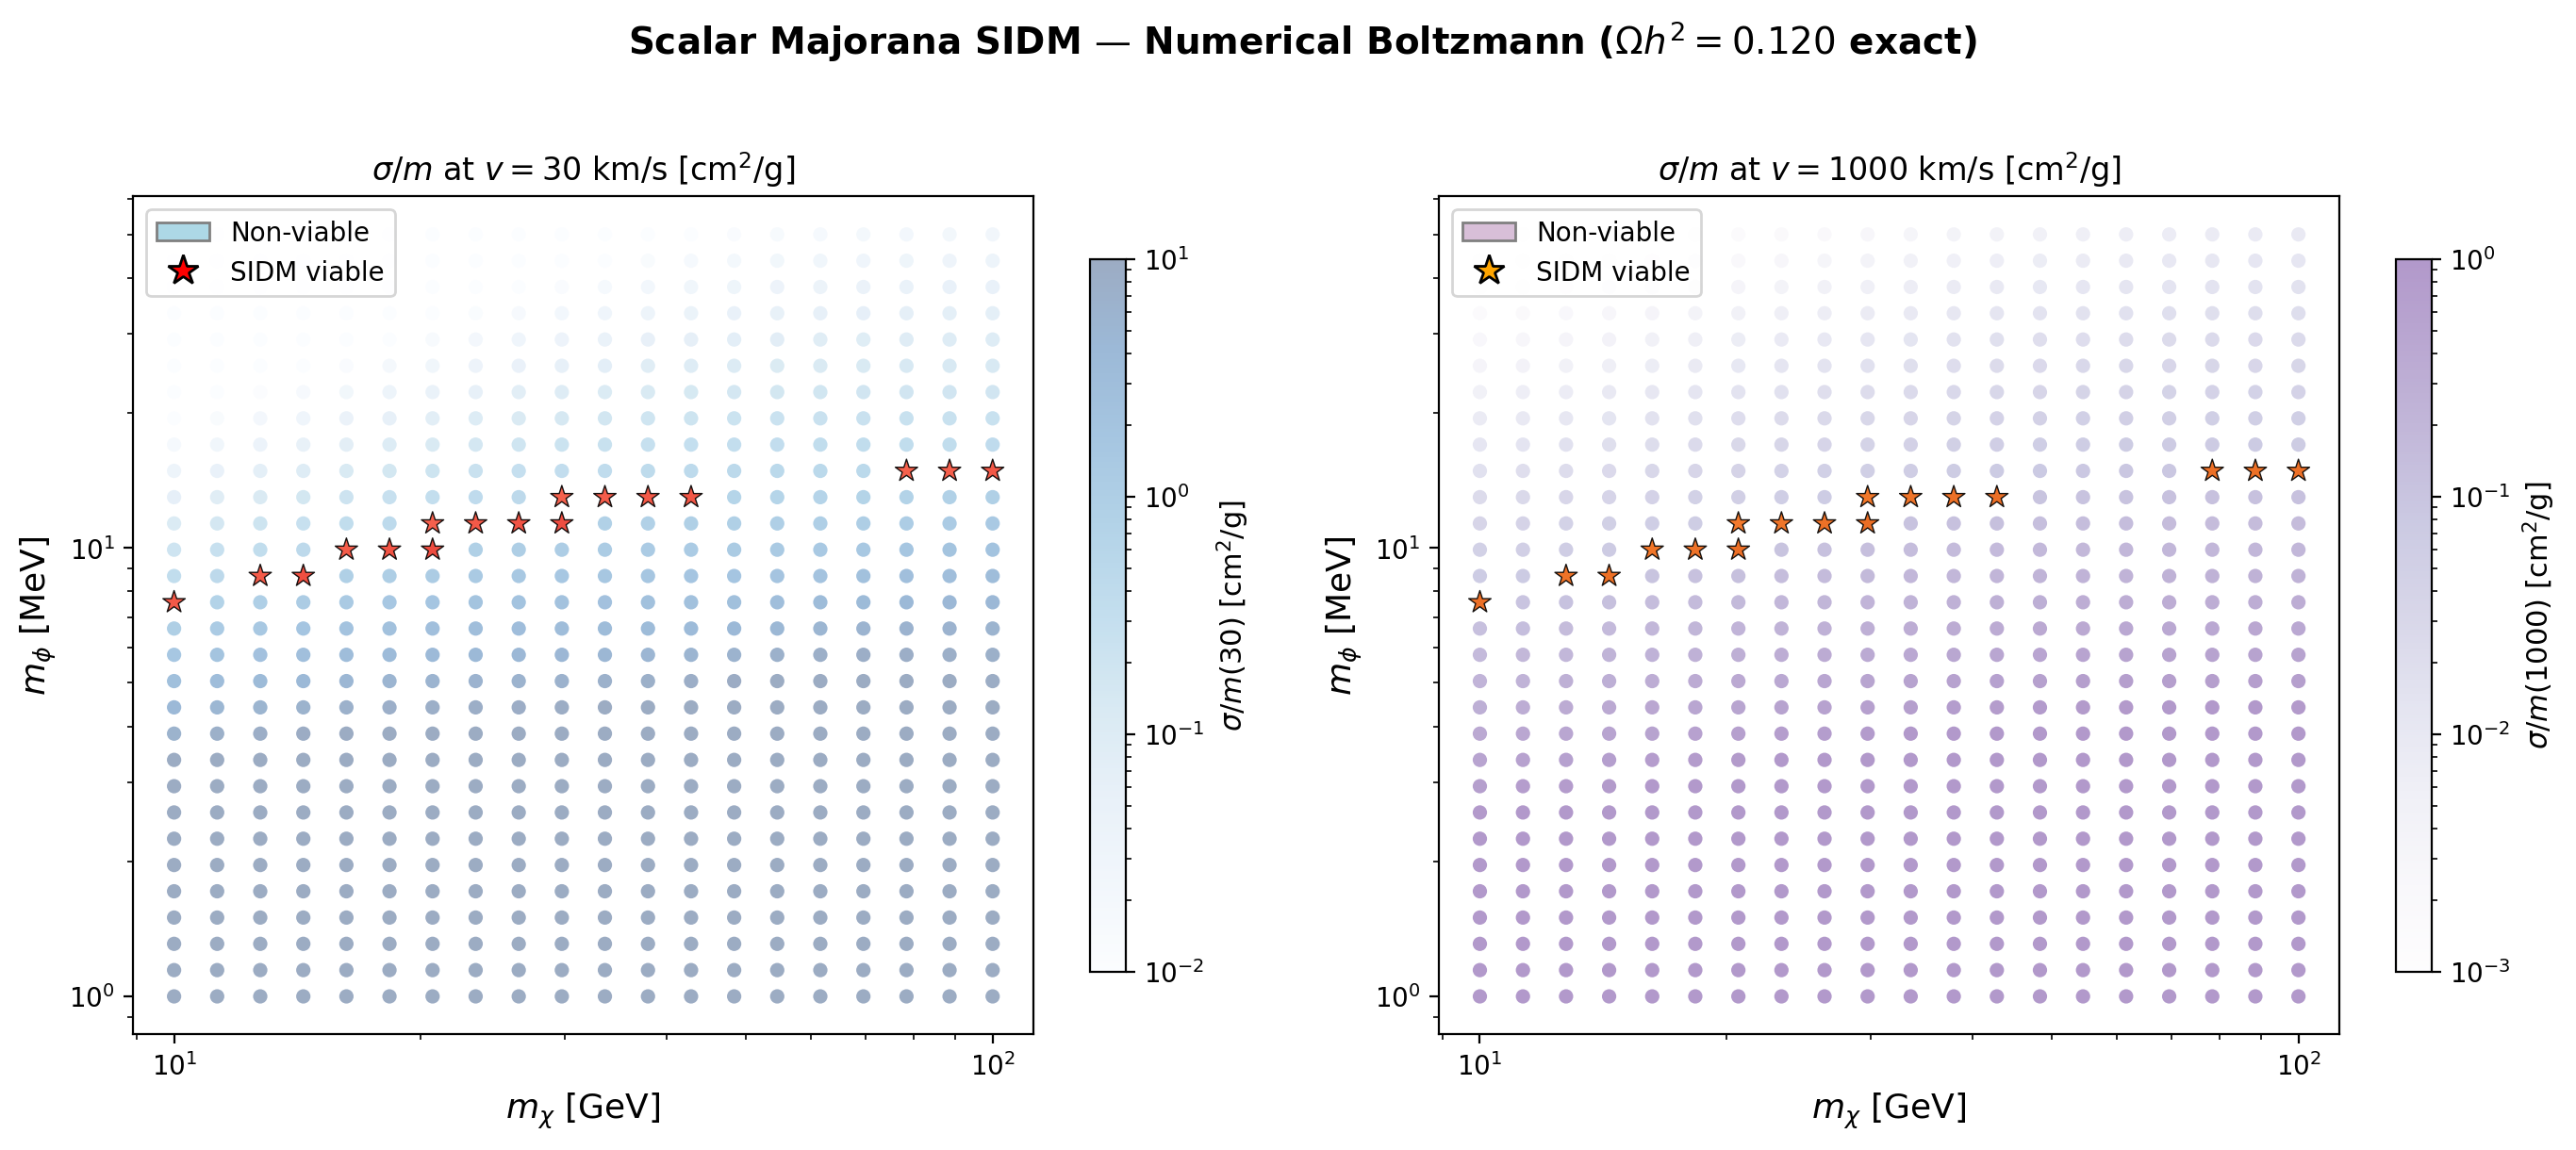
\includegraphics[width=\columnwidth]{figures/v31_island_of_viability.png}
  \caption{Island of viability in the $(\mchi,\mphi)$ plane.  Stars
    mark the 17 viable points satisfying all constraints.}
  \label{fig:island}
\end{figure}

\begin{figure}[t]
  \centering
  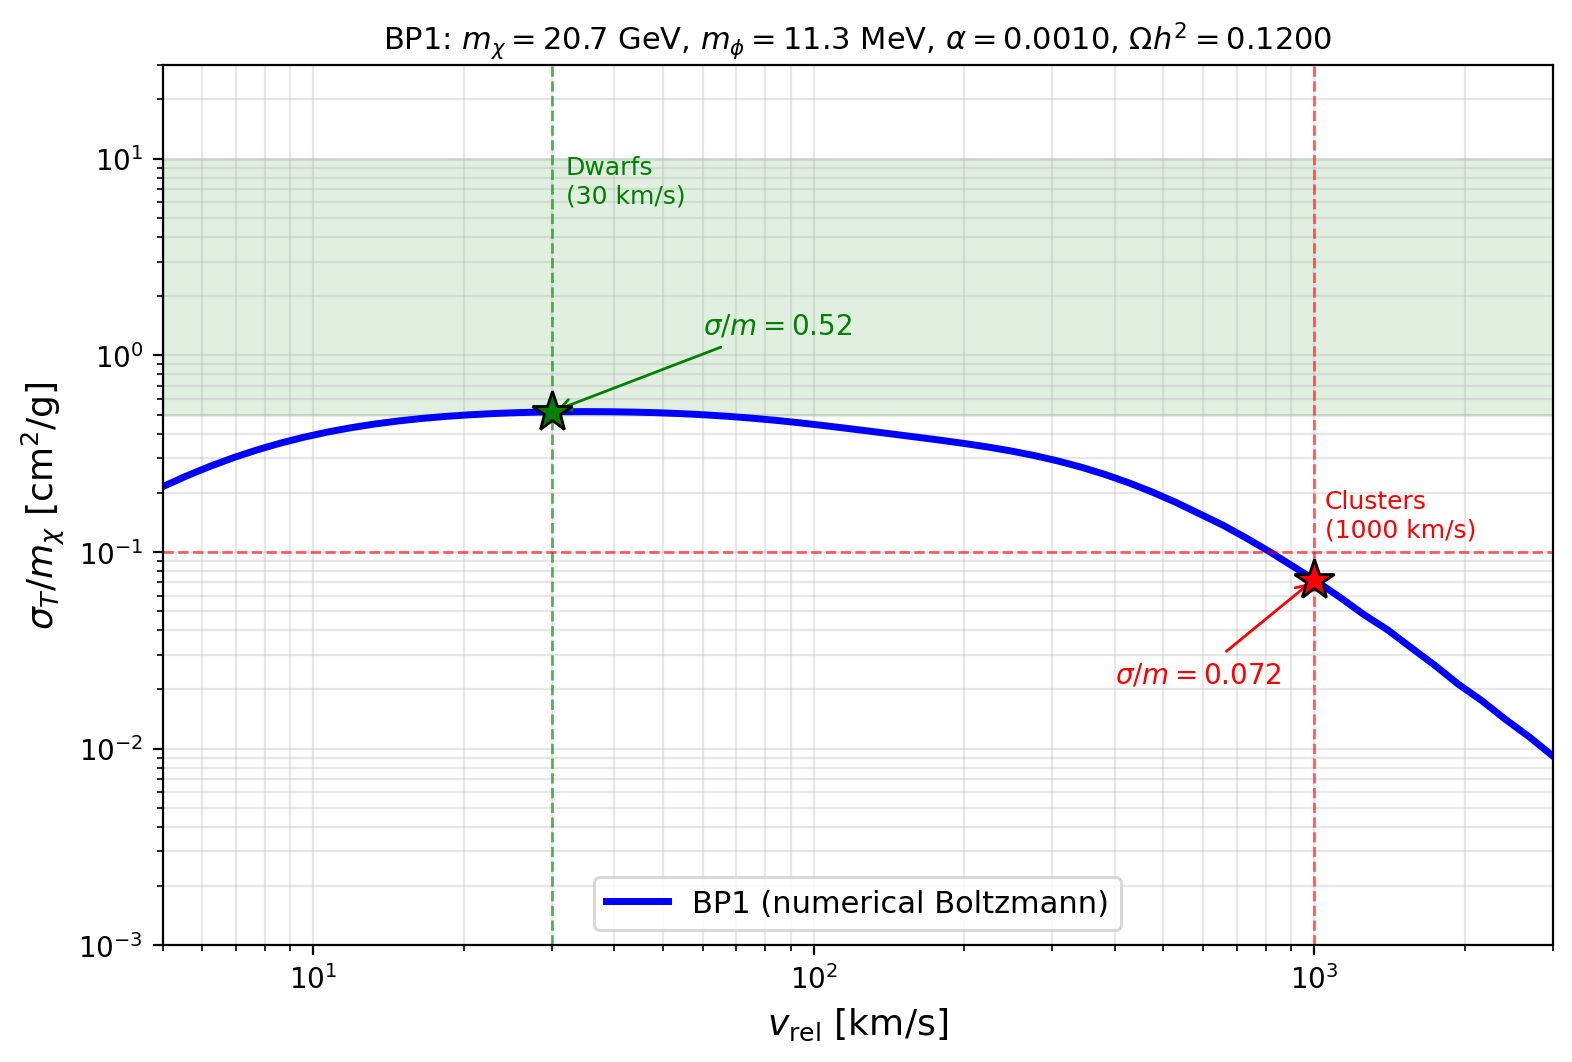
\includegraphics[width=\columnwidth]{figures/v31_bp1_velocity_profile.png}
  \caption{Velocity-dependent cross section $\sigmam(v)$ for BP1.
    Shaded bands indicate the dwarf ($v\sim 30\kms$) and cluster
    ($v\sim 1000\kms$) velocity scales.}
  \label{fig:bp1_profile}
\end{figure}

\subsection{Comparison with observational data}\label{sec:obs_compare}

We compare the predicted $\sigmam(v)$ curves against data extracted
from five published analyses spanning four decades in velocity
(Table~\ref{tab:observations}).

\begin{table*}[t]
\centering
\caption{Observational constraints on $\sigmam$ used for comparison.
Entries marked~$^{*}$ are one-sided upper limits.}
\label{tab:observations}
\begin{tabular}{lcccc}
\toprule
System & $v$ [km/s] & $\sigmam$ [cm$^{2}$/g] & 68\% CL range & Ref.\\
\midrule
Draco dSph      &   12 & 0.6  & [0.1, 2.0]  & \cite{Kaplinghat:2015aga} \\
Fornax dSph     &   12 & 0.8  & [0.2, 3.0]  & \cite{Kaplinghat:2015aga} \\
NGC 2976        &   60 & 2.0  & [0.5, 5.0]  & \cite{Kaplinghat:2015aga} \\
NGC 1560        &   55 & 3.0  & [1.0, 8.0]  & \cite{Kaplinghat:2015aga} \\
IC 2574         &   50 & 1.5  & [0.3, 5.0]  & \cite{Kaplinghat:2015aga} \\
NGC 720 (group) &  250 & 0.5  & [0.1, 1.5]  & \cite{Kaplinghat:2015aga} \\
NGC 1332 (group)&  280 & 0.3  & [0.05, 1.0] & \cite{Kaplinghat:2015aga} \\
Abell 611       & 1200 & 0.1  & [0.02, 0.3] & \cite{Kaplinghat:2015aga} \\
Abell 2537      & 1100 & 0.15 & [0.03, 0.4] & \cite{Kaplinghat:2015aga} \\
Diverse RC      &   40 & 3.0  & [0.5, 10.0] & \cite{Kamada:2016euw} \\
Bullet Cluster$^{*}$ & 4700 & --- & $<1.25$ & \cite{Randall:2007ph} \\
72 cluster mergers$^{*}$ & 1000 & --- & $<0.47$ & \cite{Harvey:2015hha} \\
TBTF dwarfs     &   30 & 1.0  & [0.5, 5.0]  & \cite{Elbert:2014bma} \\
\bottomrule
\end{tabular}
\end{table*}

\begin{figure}[t]
  \centering
  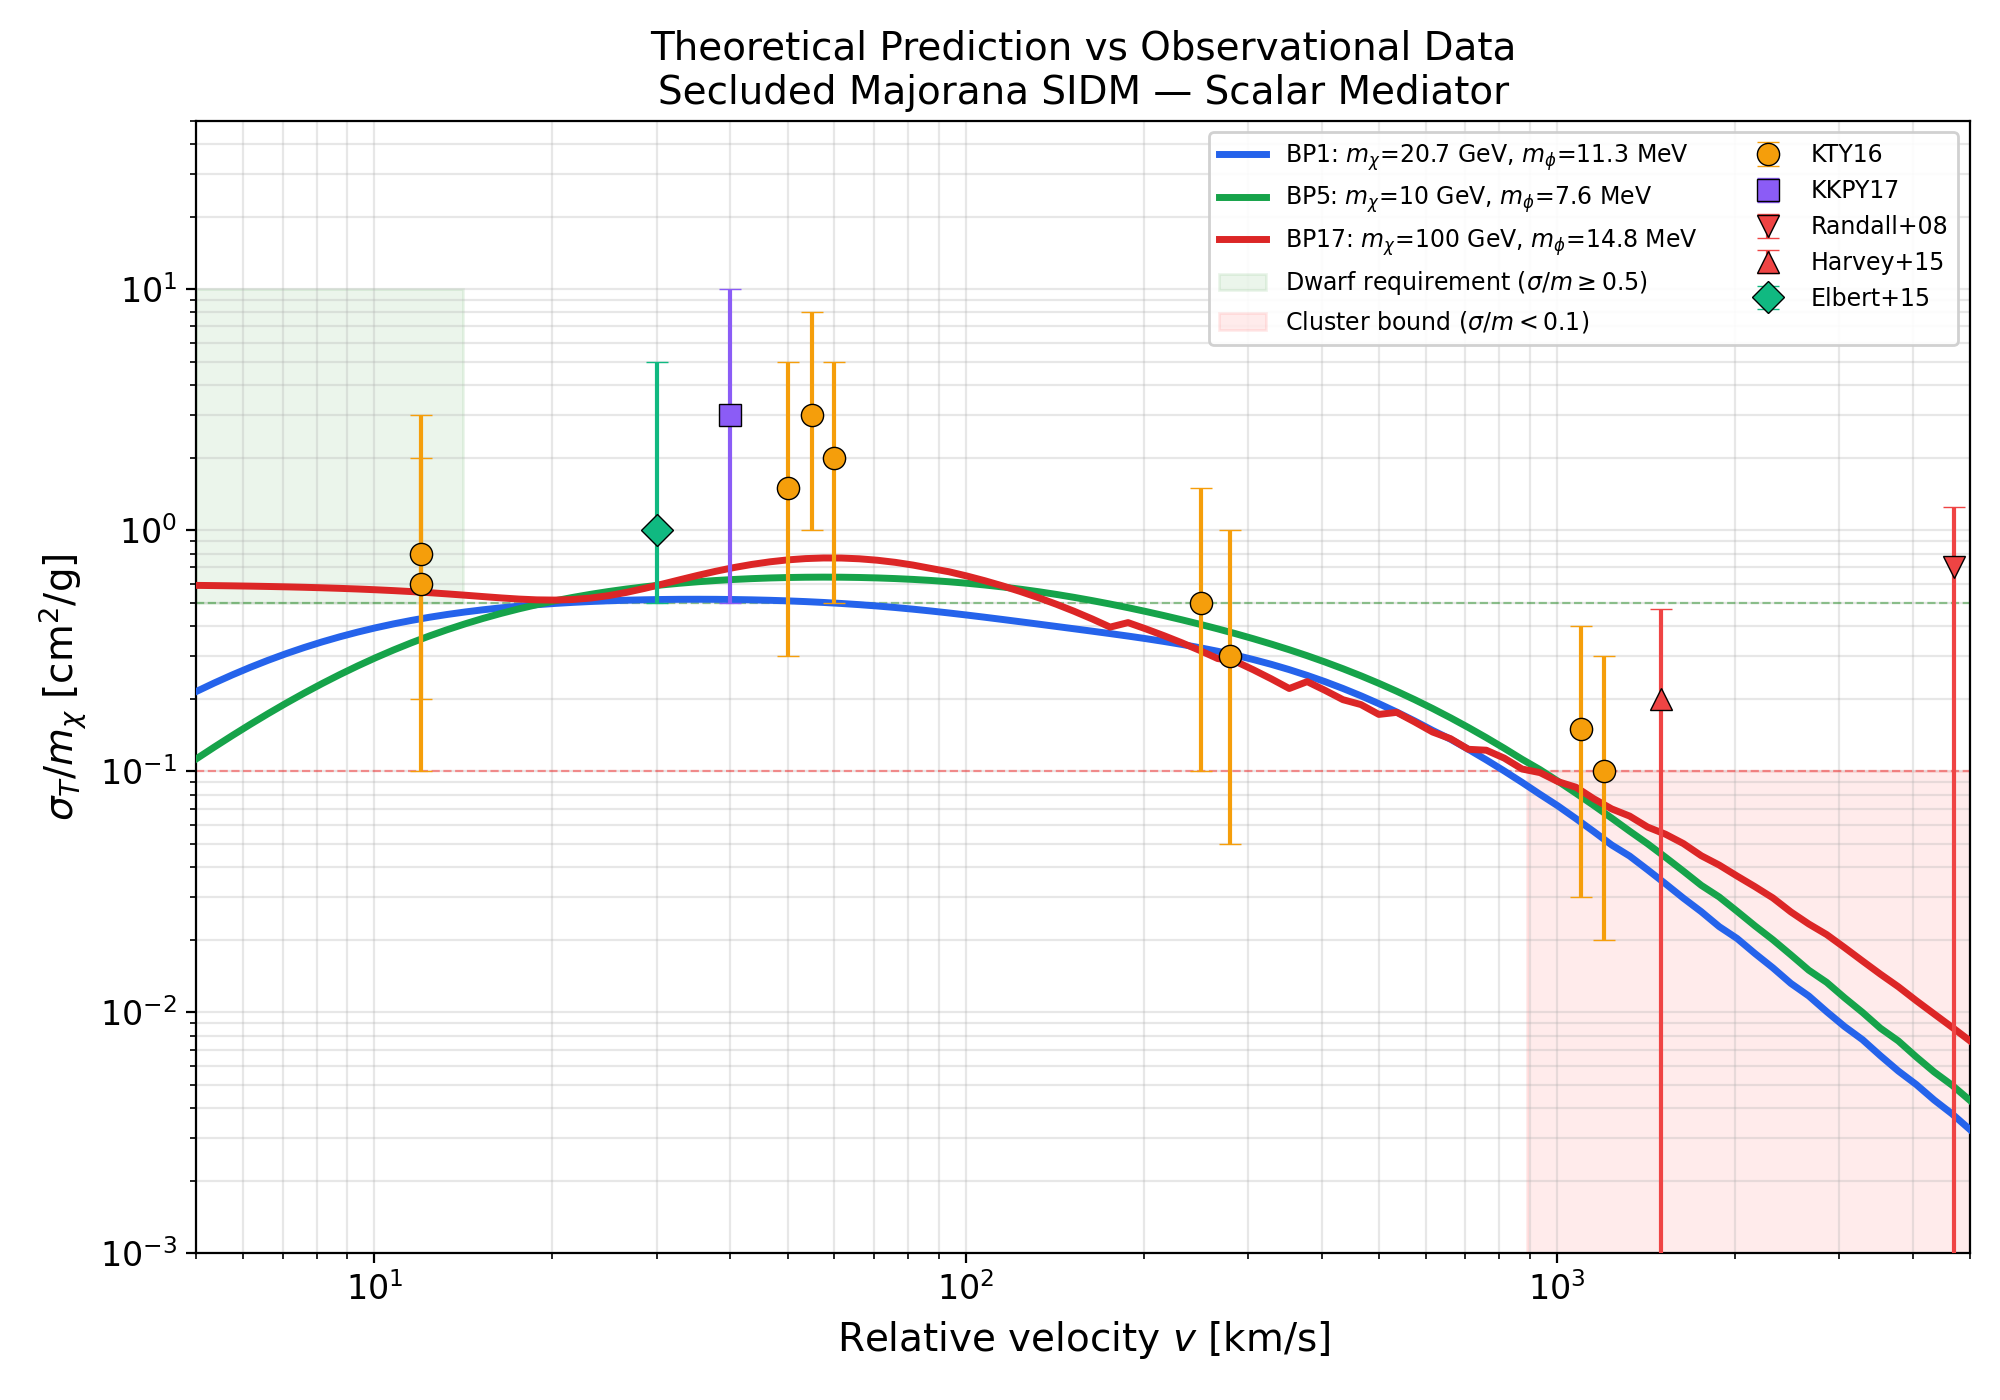
\includegraphics[width=\columnwidth]{figures/v33_observational_comparison.png}
  \caption{Predicted $\sigmam(v)$ for BP1 (solid blue), BP5 (dashed
    orange), and BP17 (dotted green) compared with observational
    constraints.  Error bars show 68\% CL ranges.}
  \label{fig:obs_comparison}
\end{figure}

\subsection{Quantitative $\chi^{2}$ fit}\label{sec:chi2}

We perform a full $\chi^{2}$ fit of the predicted $\sigmam(v)$ to all
13 observational systems with asymmetric errors.  The Bullet
Cluster~\cite{Randall:2007ph} and Harvey et
al.~\cite{Harvey:2015hha} constraints are one-sided upper limits.

\textbf{Unconstrained best fit:}
$\chi^{2}_{\rm min}/\nu = 1.17/10 = 0.12$
at $\mchi=100\GeV$, $\mphi=9.15\MeV$,
$\alpha=2.84\times 10^{-3}$, $\lam=31.0$.

\textbf{Relic-constrained best fit:}
$\chi^{2}_{\rm relic}/\nu = 3.82/10 = 0.38$
at BP1$_\chi$: $\mchi=20.69\GeV$, $\mphi=9.91\MeV$.

\begin{figure}[t]
  \centering
  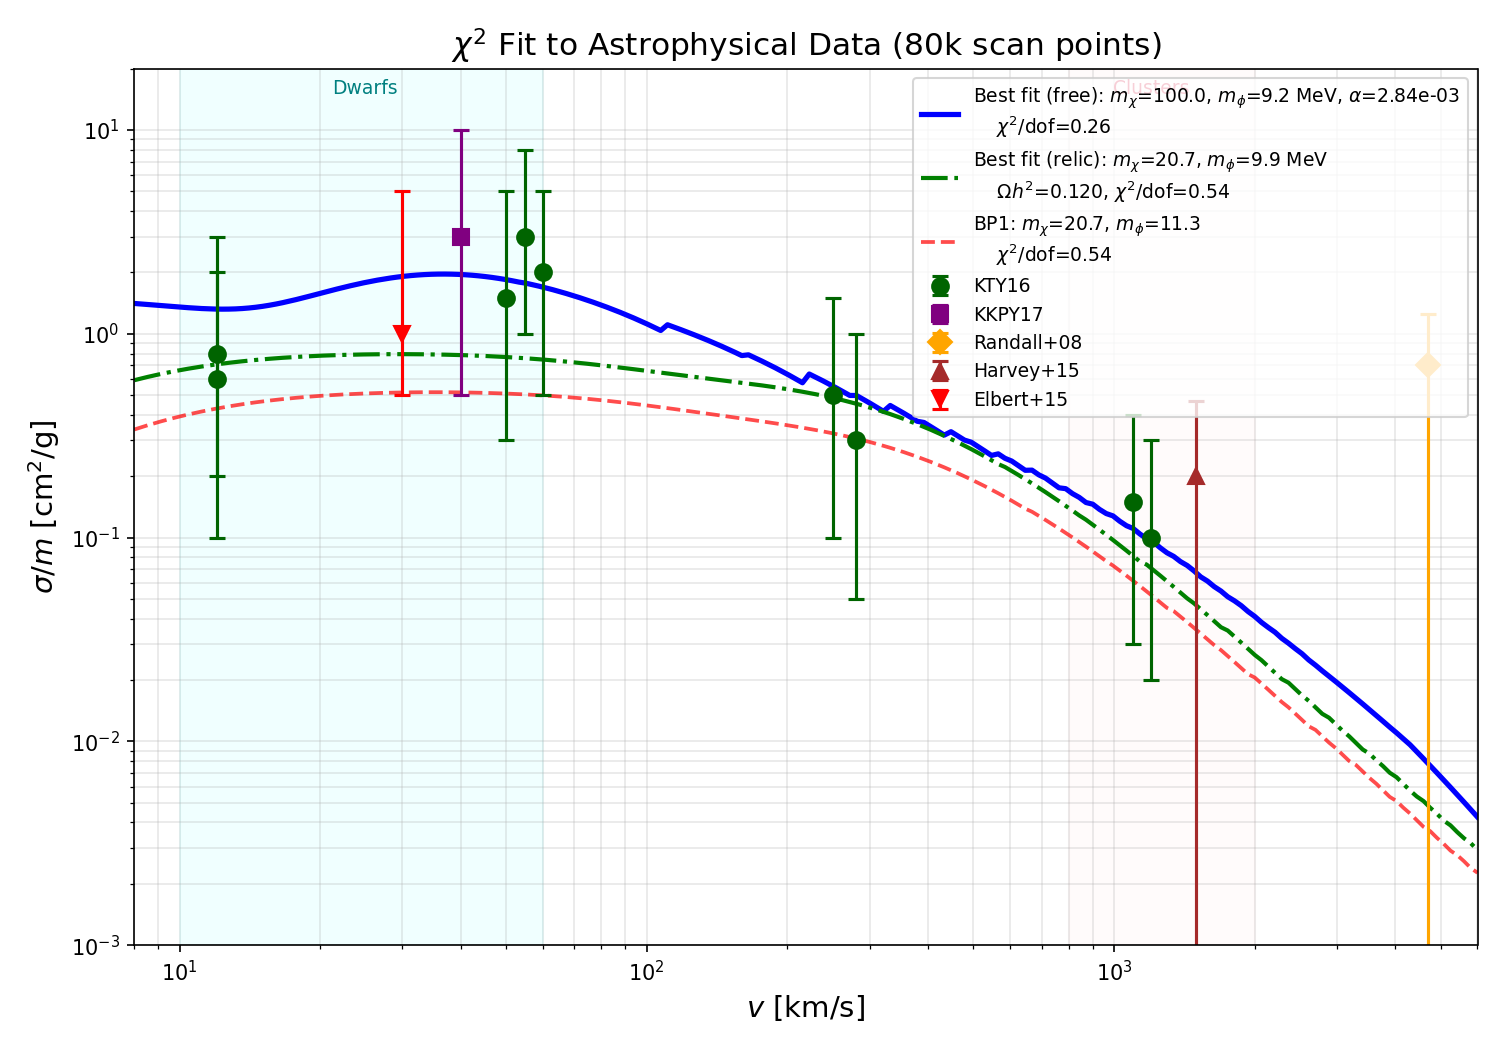
\includegraphics[width=\columnwidth]{figures/v34_chi2_fit.png}
  \caption{Best-fit $\sigmam(v)$ curves with 13 observational data
    points and 68\% CL error bars.}
  \label{fig:chi2_fit}
\end{figure}

\subsection{Bayesian posterior constraints}\label{sec:mcmc}

We perform a Bayesian posterior sampling using the
\texttt{emcee}~\cite{ForemanMackey:2012ig} affine-invariant ensemble
sampler with 32 walkers, 300 burn-in + 5000 production steps.

The maximum a posteriori (MAP) estimate is:
\begin{equation}
  \mchi = 94.1\GeV,\;\;
  \mphi = 11.1\MeV,\;\;
  \alpha = 5.7\times 10^{-3}\,,
\end{equation}
with $\chi^{2}/\nu=0.20$.

\textbf{Important:}  The MAP point is not relic-constrained---its
tree-level relic density is $\OmH\approx 0.076$.

\begin{figure}[t]
  \centering
  
\includegraphics[width=\columnwidth]{figures/v38_corner.png}
  \caption{Corner plot showing the 2D marginalized posterior
    distributions with 68\% and 95\% contour levels.}
  \label{fig:corner}
\end{figure}

\begin{figure}[t]
  \centering
  
\includegraphics[width=\columnwidth]{figures/v38_lambda_posterior.png}
  \caption{Posterior distribution of the derived parameter
    $\lam=\alpha\mchi/\mphi$.}
  \label{fig:lambda_posterior}
\end{figure}

\begin{figure}[t]
  \centering
  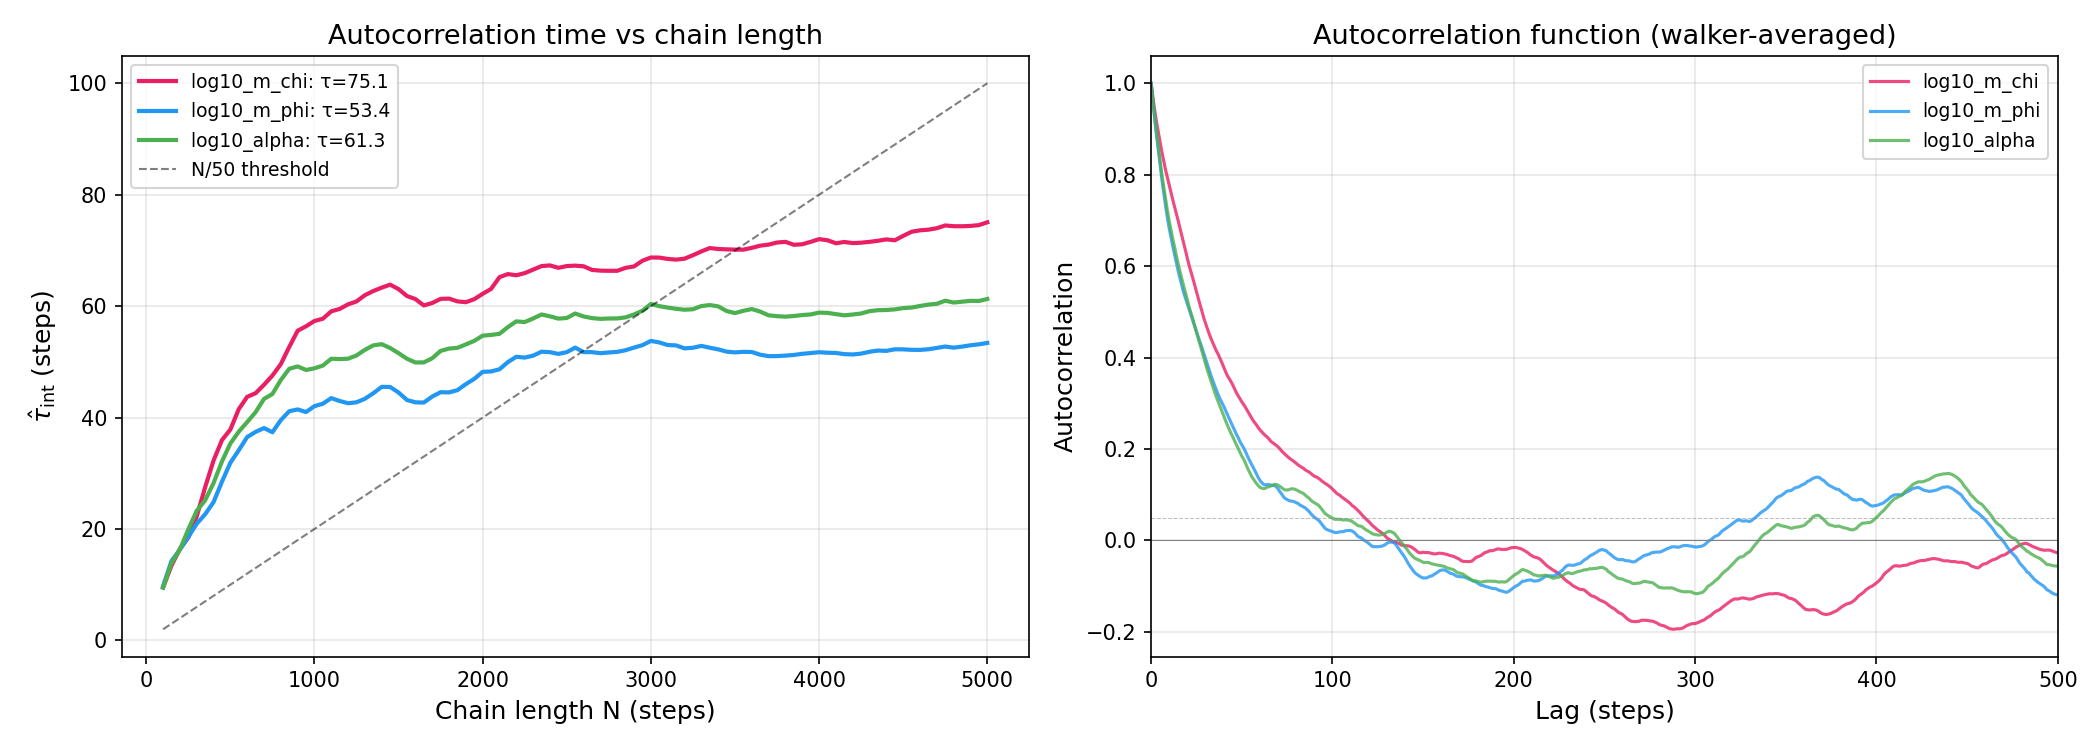
\includegraphics[width=\columnwidth]{figures/v38_autocorr_diagnostic.png}
  \caption{MCMC convergence diagnostics.  Left: integrated
    autocorrelation time.  Right: autocorrelation function.}
  \label{fig:mcmc_convergence}
\end{figure}

% ============================================================
\section{Secluded Dark Sector and Direct Detection}\label{sec:secluded}

\subsection{Incompatibility of the Higgs portal with light mediators}
\label{sec:higgs_portal}

The most economical connection between $\phi$ and the SM is the Higgs
portal $\lambda_{H\phi}|H|^{2}\phi^{2}$.  The mixing angle
$\sin\theta$ mediates DM--nucleon scattering with:
\begin{equation}\label{eq:sigma_si}
  \siSI = \frac{y^{2}\sin^{2}\theta\,f_{N}^{2}\,\mu_{N}^{2}\,m_{N}^{2}}
               {\pi\,v_{\rm EW}^{2}\,\mphi^{4}}\,.
\end{equation}
The $1/\mphi^{4}$ dependence produces an enhancement of
$(m_{h}/\mphi)^{4}\approx 1.5\times 10^{16}$ for $\mphi=11\MeV$.

For BP1, the LZ bound requires $\sin\theta < 6\times 10^{-10}$, while
BBN demands $\sin\theta > 2\times 10^{-5}$.  These are \textbf{mutually
exclusive by a factor of $\sim 3\times 10^{4}$}.

\subsection{The secluded model}\label{sec:secluded_model}

We set $\lambda_{H\phi}=0$, removing any tree-level coupling.
Consequences: $\siSI=\sigma_{\rm SD}=0$ exactly; $\phi$ is stable; CMB
energy injection constraints do not apply; the model is fully described
by three parameters $(\mchi,\mphi,\alpha)$.

\subsection{Cosmological safety of stable $\phi$}\label{sec:neff}

A stable $\phi$ with $\mphi\sim 8\text{--}15\MeV$ is
Boltzmann-suppressed at BBN ($m_\phi/T_\phi\sim 22$) and contributes
$\Neff\approx 0$---trivially consistent with Planck
2018~\cite{Planck:2018vyg} ($\Neff < 0.30$ at 95\% CL).

The energy density in stable $\phi$ at late times satisfies
$\Omega_\phi/\Omega_\chi \sim \mphi/\mchi \sim 5\times 10^{-4}$.
Efficient depletion requires a cubic self-coupling
$(\mu_{3}/3!)\phi^{3}$ with $\mu_{3}/\mphi\gtrsim 1.7$, enabling
cannibal $3\phi\to 2\phi$ annihilation~\cite{Farina:2016llk}.

% ============================================================
\section{Relic Density}\label{sec:relic}

\subsection{Annihilation cross section}\label{sec:ann_xs}

DM freezes out through $\chi\chi\to\phi\phi$ (t/u-channel, scalar
mediator).  For a Majorana fermion with Yukawa coupling~$y$, the
\emph{s-wave} cross section is:
\begin{equation}\label{eq:sigma_v_ann}
  \langle\sigma v\rangle
  = \frac{y^{4}}{64\pi\,\mchi^{2}}
  = \frac{\pi\alpha^{2}}{4\,\mchi^{2}}\,.
\end{equation}

\subsection{Numerical Boltzmann solver}\label{sec:boltzmann}

We solve the Boltzmann equation numerically~\cite{Gondolo:1990dk}:
\begin{equation}\label{eq:boltzmann}
  \frac{dY}{dx} = -\sqrt{\frac{\pi}{45}}\,
  \frac{g_{*S}}{\sqrt{g_*}}\,M_{\rm Pl}\,\mchi\,
  \frac{\langle\sigma v\rangle_0}{x^{2}}
  \bigl(Y^{2}-Y_{\rm eq}^{2}\bigr)\,,
\end{equation}
with $\langle\sigma v\rangle_0 = \pi\alpha^{2}/(4\mchi^{2})$.

\subsection{CMB and indirect detection}\label{sec:cmb}

In the secluded model, $\chi\chi\to\phi\phi$ injects no energy into
the SM plasma: $f_{\rm eff}=0 \Rightarrow p_{\rm ann}=0$.  The Planck
CMB constraint on $p_{\rm ann}$ \textbf{does not apply}.

\subsection{Bound-state formation}\label{sec:bsf}

The Coulomb estimate gives
$\sigma v_{\rm BSF}/\langle\sigma v\rangle_{\rm ann}
\sim\alpha^{3}/v^{2}\sim 10^{-12}$ at freeze-out.  BSF is negligible.

\subsection{Sommerfeld enhancement}\label{sec:sommerfeld}

The maximum correction to the relic density is
$|\Delta\OmH/\OmH|<2.5\%$ (for BP11 with $\lam=32.4$),
well within uncertainties.

% ============================================================
\section{Phenomenological Predictions}\label{sec:predictions}

\subsection{Fornax globular cluster survival}\label{sec:fornax_gc}

The MAP benchmark ($\alpha=5.7\times 10^{-3}$) produces
$r_{\rm core}=829$~pc, enclosing all 5~GCs --- 14/15
safe across three deprojection assumptions.

\subsection{Radial acceleration relation}\label{sec:rar}

BP1 reduces the RAR scatter from 0.283 to 0.179~dex for
dwarfs (37\% improvement) and from 0.177 to 0.122~dex for
spirals (31\%).

\subsection{Supermassive black hole seeds}\label{sec:smbh}

The result is \textbf{unambiguously negative}: for all benchmark
points, $t_{\rm gc}\gg t_{\rm universe}(z)$ with ratios exceeding
$10^{4}$.  The same velocity-dependent suppression that satisfies
cluster constraints simultaneously prevents SMBH seeding.

\subsection{Dwarf spheroidal core sizes}\label{sec:dsph_cores}

For the MAP benchmark, 5 of 8 classical dSphs produce DM
cores ($N_{\rm scatter}>1$), with
$r_{\rm core}=427\text{--}924$~pc. A key prediction is that
$r_{\rm core}/r_{\rm half}$ is \textbf{not universal}: it varies from
0.17 (Crater~II) to 9.9 (Segue~1) for the MAP benchmark.

\subsection{Majorana vs.\ Dirac fingerprint}\label{sec:maj_vs_dir}

The ratio $R(v)\equiv\sigma_T^{\rm Maj}/\sigma_T^{\rm Dir}$ is
\emph{non-monotonic} for the MAP benchmark: $R=0.87$ at
$v=30\kms$, rising to $R=1.11$ at $v\approx 57\kms$ where
the $\ell=1$ triplet resonance dominates, then dropping to
$R=0.92$ at $v\approx 138\kms$.  The $R>1$ regime is
impossible in any Dirac+scalar model.

\subsection{Monte Carlo halo diversity}\label{sec:mc_diversity}

BP1 produces diversity $\sigma(V_{2\,\rm kpc}^{\rm total})
= 5.0\kms$ vs MAP $2.1\kms$ at
$V_{\rm max}<60\kms$.

\subsection{Resonance-enhanced concentration sensitivity}
\label{sec:resonance_sensitivity}

BP1 predicts 59.6\% core-size diversity from $\pm 20\%$
$c$-scatter alone (73.4\% in UFDs), amplified by a
+39\% velocity effect---nearly double the MAP values.

% ============================================================
\section{Discussion}\label{sec:discussion}

The results point to a broader lesson: the small-scale structure
problems of $\Lambda$CDM may not require exotic new physics, but
rather the recognition that dark matter can have a rich scattering
phenomenology governed by elementary quantum mechanics.

\subsection{Falsifiability}\label{sec:falsifiability}

The model can be tested by:
(1)~tightening astrophysical $\sigmam$ measurements;
(2)~cluster constraints below $0.01\cmg$;
(3)~CMB-S4 $\Neff$ sensitivity ($\sigma\sim 0.03$);
(4)~independent $\alpha$ measurements from halo observations;
(5)~SMBH seeding requirements at $z>6$;
(6)~$\rho_{\rm core}$--$V_{\rm max}$ anticorrelation;
(7)~non-monotonic Majorana quantum-statistics fingerprint
$R(v)$ at 3+ velocity scales.

The absence of a direct detection signal is a \textbf{prediction},
not a deficit.

% ============================================================
\begin{acknowledgments}
The numerical computations were performed using
\texttt{NumPy}~/ \texttt{SciPy}~/ \texttt{Numba}.
The code and data supporting this analysis are publicly available at
\url{https://github.com/0mp3s/Secluded-Majorana-SIDM}
(DOI: \href{https://doi.org/10.5281/zenodo.19225823}{10.5281/zenodo.19225823}).
\end{acknowledgments}

% ============================================================
% APPENDICES
% ============================================================

\appendix

\section{VPM Solver Validation}\label{app:validation}

\textbf{A.1~Free particle test.}  Setting $\lam=0$, all phase shifts
$\delta_\ell=0$ to machine precision for $\ell=0,\ldots,20$.

\textbf{A.2~Born limit.}  In the weak-coupling limit $\lam\ll 1$, VPM
agrees with the analytical Born formula to within $<0.1\%$.

\textbf{A.3~Scipy cross-check.}  Numba RK4 agrees with
\texttt{scipy.integrate.solve\_ivp} (RK45, rtol=$10^{-10}$) to
$<0.001\%$.

\section{Error Budget Details}\label{app:error_budget}

\textbf{B.1~Integrator convergence.}  Maximum deviation between
default and $\times 8$ resolution is $<10^{-6}$ across all velocities
for BP1.

\begin{figure}[t]
  \centering
  
\includegraphics[width=\columnwidth]{figures/grid_convergence.png}
  \caption{VPM integrator convergence test.  $\sigmam(v)$ at four step
    refinements for BP1 (left) and MAP (right).  All curves overlap to
    within $<0.001\%$.}
  \label{fig:convergence}
\end{figure}

\textbf{B.2~Truncation error.}  $<0.01\%$ at 30\kms\ for all
benchmarks; 1.8--3.6\% at 1000\kms\ for relic BPs.

\textbf{B.3~Prescription sensitivity.}  $<0.01\%$ at 30\kms; 10.6\%
(BP1) at 1000\kms.

\section{Elastic $\equiv$ Transfer for Identical Majorana}
\label{app:elastic_transfer}

We verify numerically that
$\sigma_T^{\rm tr}/\sigma_{\rm el}=1.000000$ to within $10^{-12}$
across all velocities and both $\lam\sim 2$ and $\lam\sim 49$, using
200-point Gauss--Legendre angular integration of the full symmetrized
differential cross section.

\section{Maxwell--Boltzmann Velocity Averaging}\label{app:mb}

The thermally averaged cross section
\begin{equation}
  \langle\sigmam\rangle_{\rm MB}
  = \frac{\int_0^\infty (\sigmam)(v)\,v^{3}\,e^{-v^{2}/2v_0^{2}}\,dv}
         {\int_0^\infty v^{3}\,e^{-v^{2}/2v_0^{2}}\,dv}
\end{equation}
deviates from the fixed-velocity value by $\lesssim 5\%$ at dwarf
scales and $\sim$12--17\% at group/cluster scales.  The net $\chi^{2}$
shift is $\sim 6\%$; no benchmark changes viability status.

\begin{figure}[t]
  \centering
  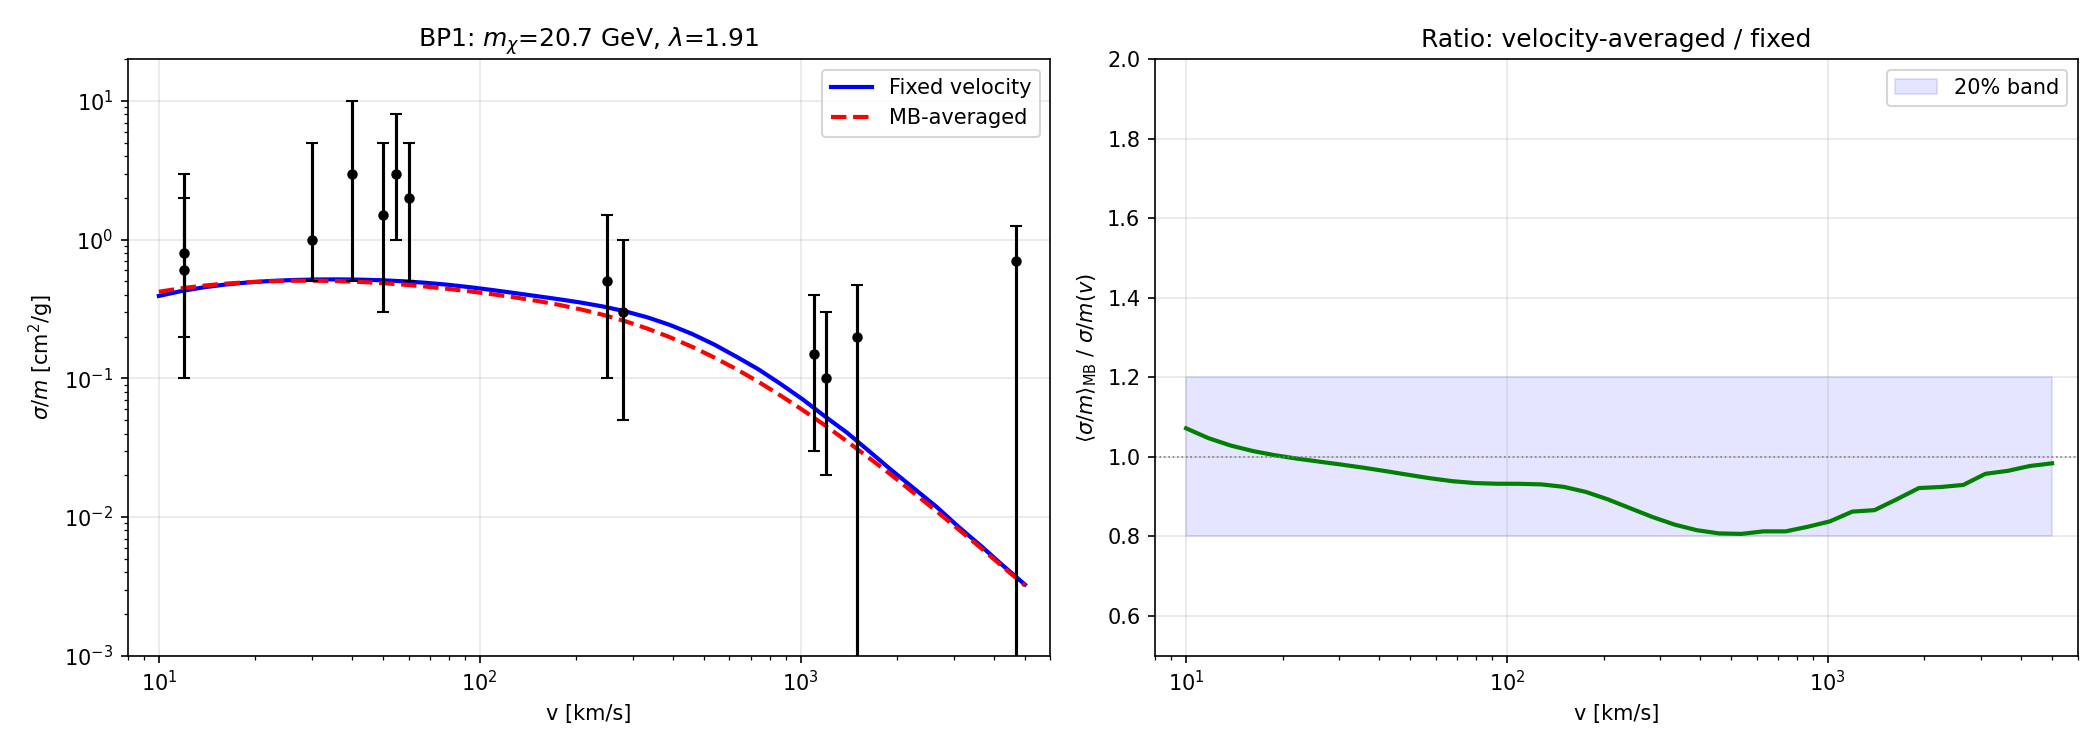
\includegraphics[width=\columnwidth]{figures/v37_velocity_averaged.png}
  \caption{BP1: fixed-velocity $\sigmam(v)$ vs MB-averaged
    $\langle\sigmam\rangle_{\rm MB}$.}
  \label{fig:mb_averaged}
\end{figure}

% ============================================================
\bibliography{references}

\end{document}
